\documentclass{article}
\usepackage{graphicx}
\usepackage{amsmath,amssymb}
\usepackage{booktabs}
\usepackage{hyperref}
\graphicspath{{../reference/paper-figures/}}

\title{Recurrent Depth in Z1T: An Empirical Quality--Storage Trade-off}
\author{Kirk Stapff}
\date{September 2026}

\begin{document}

\maketitle

\begin{abstract}
Accelerators that store a sparse program on-chip make unique body weights a first-class cost: extra unique depth requires extra couplings or extra reprogramming, whereas extra applied depth can reuse a resident core. We study that trade-off in Extropic's Z1T recipe by comparing three models that isolate storage from execution: six unique residual blocks applied once (U6), the same six blocks applied twice (R6$\times$2), and twelve unique blocks applied once (U12). Models share width, sparsity, tokenizer, and a matched budget of $254{,}164{,}992$ target-token presentations. We estimate two contrasts on an OpenWebText-subset holdout with six independent training seeds. At identical unique body capacity ($102{,}589$ parameters), R6$\times$2 improves over U6 by $2.35\%$ perplexity (mean NLL gap $-0.0237$~nats/token; $97.5\%$ paired interval $[-0.0273,-0.0202]$). At matched applied depth $12$, sharing costs $0.81\%$ perplexity versus U12 while using $49.8\%$ fewer unique body parameters (mean gap $+0.0081$; interval $[+0.0023,+0.0139]$). These results support a quality--storage trade-off in the tested regime; whether resident reuse reduces deployment energy depends on program-loading and execution costs.
\end{abstract}

\section{Introduction}

Accelerators that retain sparse programs on-chip motivate a distinction between unique model capacity and applied computation. A deeper untied network requires additional unique weights, whereas a recurrent network can repeatedly apply a smaller stored core. When a model exceeds resident capacity, additional program loading may introduce latency and energy costs. Whether weight sharing provides a useful alternative depends both on its effect on language-model quality and on the deployment schedule.

We investigate this trade-off in the Z1T software architecture. We compare six unique residual blocks applied once (U6), the same six blocks applied twice (R6$\times$2), and twelve unique blocks applied once (U12). These comparisons measure the benefit of additional computation at fixed unique-body capacity and the cost of sharing at fixed applied depth. Our contributions are (1)~a reproducible three-arm Z1T evaluation, (2)~a six-seed held-out estimate of these two effects, and (3)~a conditional analysis of program loading under a six-block residency constraint.

\section{Related Work}

Universal Transformers repeatedly apply a shared transformation to sequence representations~\cite{dehghani2019}, while ALBERT uses cross-layer sharing to reduce parameter count~\cite{lan2020}. Geiping et al.\ increase test-time computation through recurrent latent depth without generating additional text tokens~\cite{geiping2025}. These precedents establish that unique parameter capacity and applied depth can be varied separately; recurrence itself is not new. Our contribution is not weight tying, but a controlled evaluation of its quality--storage trade-off in Z1T. Our recurrent model is compared with both an untied model of equal unique-body capacity and one of equal applied depth.

Coconut instead feeds hidden states back as subsequent input embeddings, bypassing intermediate word decoding~\cite{hao2024}. Our study addresses more narrowly what effect repeated block applications can have on next-token prediction when comparing controls matched on either unique body capacity or applied depth. We train and evaluate each architecture at a fixed recurrence count; we do not measure adding inference passes to an already-trained model.

Attention-free transformers replace dot-product attention with gated aggregation; AFT-conv incorporates locality while retaining global connectivity~\cite{zhai2021}. We build on Extropic's Z1T software recipe for sparse language modeling~\cite{extropic2026z1t}, rather than introducing a new sequence mixing operator. Amico et al.\ distinguish inexpensive Gibbs updates under fixed couplings from more costly readout and program flashing on Z1~\cite{amico2026}. They report an energy ordering on Z1 (sample $\ll$ read $\ll$ flash); we use that ordering as motivation, not as a measurement of recurrent Z1T. We measure language-model quality and unique body storage in software, and derive conditional reload-cost break-even conditions under an explicitly assumed deployment schedule.

\section{Model and Comparisons}

We start from the published Z1T stack and introduce looping of residual blocks. The rest of the architecture is inherited: token embedding, additive sinusoidal positional encoding, a stack of residual blocks, a final Dynamic Tanh (DyT)~\cite{zhu2025}, and a dense vocab classifier. Each block is
\[
x \leftarrow x + \mathrm{AFTConv}(\mathrm{DyT}(x)),
\qquad
x \leftarrow x + \mathrm{MLP}(\mathrm{DyT}(x)).
\]
AFTConv is the Z1T implementation of causal AFT-conv~\cite{zhai2021}: sparse projections, a causal depthwise convolution of kernel size $4$, and a causal cumulative pool of the same streams. Linear maps in the body use fan-in $c=4$ with a fixed random gather. Every body affine is tanh-wrapped; the MLP additionally uses expansion ratio $4$ and a tanh intermediate activation after the first wrapped projection. The classifier is dense and not tanh-wrapped. Width is $d=384$, sequence length is $256$, with eight AFT heads and GPT-2 BPE ($V=50{,}257$).

Let \(F_\theta\) denote the stored six-block residual stack. Recurrent execution is
\[
h^{(0)}=\mathrm{PE}(\mathrm{Embed}(x)),
\qquad
h^{(j+1)}=F_\theta\bigl(h^{(j)}\bigr),\quad j=0,\ldots,k-1,
\]
followed by the final DyT and classifier. There is no input injection: later applications see only the residual stream from the previous pass, not a fresh mix of the token embedding. Weight tying stores one Equinox parameter tree and reuses it. Teacher-forced execution recomputes convolution and cumulative pooling separately at each applied-depth position. A streaming implementation would require distinct histories at those positions even when weights are shared; cached decoding is not evaluated here.

We compare three models that isolate storage from execution (\(p=q=0\)):

\begin{figure}[t]
\centering
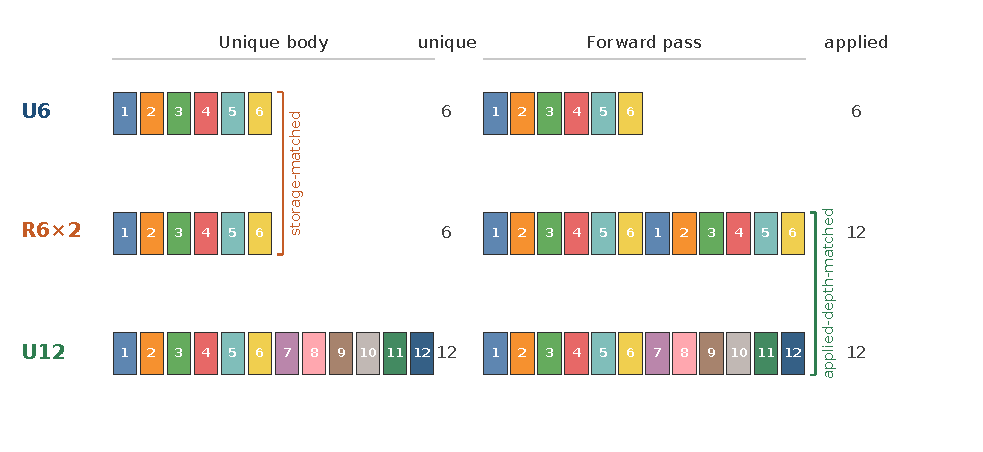
\includegraphics[width=\linewidth]{fig1-architecture.pdf}
\caption{Controlled contrasts. U6 stores and applies six unique residual blocks.
R6$\times$2 stores the same six blocks and applies them twice. U12 stores twelve unique
blocks and applies them once. Embedding and classifier are identical in structure
across arms. Diagram only.}
\label{fig:architecture}
\end{figure}

\begin{table}[t]
\centering
\caption{Architecture accounting. Body parameters exclude embedding and classifier and include the shared final DyT. Total trainable parameters include embedding ($19{,}298{,}688$) and classifier ($19{,}348{,}945$). All arms use $254{,}164{,}992$ training-token presentations.}
\label{tab:models}
\begin{tabular}{lrrrr}
\toprule
Model & Unique & Applied & Body params & Total trainable \\
\midrule
U6 & 6 & 6 & $102{,}589$ & $38{,}750{,}222$ \\
R6$\times$2 & 6 & 12 & $102{,}589$ & $38{,}750{,}222$ \\
U12 & 12 & 12 & $204{,}409$ & $38{,}852{,}042$ \\
\bottomrule
\end{tabular}
\end{table}

Body parameters are the optimizer-partitioned trainable arrays including the final DyT and excluding the token embedding and classifier. Fixed positional encoding and gather indices are not counted as trainable. Recurrence halves unique body storage, not the whole model.

U6 versus R6$\times$2 asks whether a second application of the same weights improves quality at fixed unique body storage. R6$\times$2 versus U12 asks how much quality is lost by sharing at matched applied depth $12$. Each architecture is trained separately at its evaluation recurrence count. For each training seed, U6 and R6$\times$2 share stored initialization, including sparse gather indices. Matching numeric seed IDs does not give U12 the same embedding initialization, because the upstream key allocation depends on unique depth.

\section{Experimental Setup}

We train and evaluate on an archived sample of the first $40$k nonempty streaming OpenWebText documents, tokenized with the original GPT-2 BPE vocabulary ($V = 50{,}257$). Documents are assigned to non-overlapping train, development, calibration, and confirmation splits at preparation time. We check exact-text disjointness across splits; that does not establish near-duplicate removal. This is not a corpus-wide representative sample.

Each example contains $257$ consecutive document-local tokens (256 inputs and shifted next-token targets) with stride $257$. Incomplete suffixes are discarded; documents shorter than $257$ tokens yield no windows; no EOS token is appended. Each window resets positional encoding and AFT state. Training samples eligible windows uniformly with replacement; evaluation exhausts them. The training split has $37{,}551{,}616$ eligible target positions, so $254{,}164{,}992$ presentations are repeated exposure, not distinct corpus tokens.

The primary evaluation corpus is the confirmation split, created at preparation. It comprises $788$ documents and $3{,}166$ eligible windows ($810{,}496$ scored next-token positions). A local protocol file previously listed $811{,}456$ targets; that count is a transcription error ($3{,}166\times 256=810{,}496$). We report mean negative log-likelihood in nats per token.

All models use width $d=384$, fan-in $c=4$, $8$ AFT heads, and convolution kernel size $4$. Unique trainable body parameters are $102{,}589$ for U6 and R6$\times$2 and $204{,}409$ for U12 (Table~\ref{tab:models}).

Each run used the same training recipe of AdamW with peak learning rate $3\times 10^{-4}$, weight decay $0.1$, $\beta = (0.9, 0.95)$, gradient clip $1.0$, $100$-step linear warmup, and cosine decay to $0.1\times$ peak over the full horizon. We train for $15{,}513$ steps at batch size $64$. Arms are matched on training-token presentations, not on unique corpus coverage and not on an audited FLOP total. Recurrence is trained with full backpropagation through the repeated stack. Model arrays used float32 with JAX's default matrix-multiplication precision setting (\texttt{jax\_default\_matmul\_precision=None}); full IEEE float32 multiplication was not separately enforced or audited.

During training we evaluate the confirmation split every $1{,}000$ steps and at the final step, and we record a fixed training probe for diagnostics. Primary outcomes use only the final checkpoint. We do not select the best intermediate confirmation NLL and do not call the procedure blinded.

We use six independent training seeds \(\{7,\ldots,12\}\). The same seed ID shares the training data stream across the three arms. For each seed \(i\) and control \(\in\{\mathrm{U6},\mathrm{U12}\}\) we form
\[
D_i=\mathrm{NLL}(\mathrm{R6}\times 2)_i-\mathrm{NLL}(\mathrm{control})_i
\]
and report
\[
\overline{D}\ \pm\ t_{5,\,0.9875}\,\frac{s_D}{\sqrt{6}},
\]
i.e.\ two-sided $97.5\%$ paired Student-$t$ intervals, Bonferroni over two contrasts at familywise $\alpha=0.05$. Training seeds are the replication units. The $810{,}496$ scored tokens are not independent training replicates. Intervals describe training-seed variability conditional on the fixed evaluation corpus, not uncertainty across datasets. The small sample limits assessment of the approximate-normality assumption.

The architecture and training horizon were selected using development experiments (Appendix~\ref{app:history}). A separate calibration assessment used seeds $4$--$6$. Before the final study, we specified the three-arm comparison, training horizon, seeds $7$--$12$, and final-checkpoint endpoints in archived local protocol files; this was not an external preregistration. Calibration and development outcomes are not pooled with the final estimates.

All $18$ runs used NVIDIA H100 GPUs with the same software environment (Appendix~\ref{app:env}). One registered U12 seed-$12$ run was retrained under the same identity after an infrastructure archive failure; it is not a replacement seed.

\section{Results}

Recurrent depth recovers most of the measured benefit of twelve unique blocks while storing only six unique residual blocks. On the held-out OpenWebText subset, R6$\times$2 reduces perplexity by $2.35\%$ relative to U6 at identical unique body capacity (mean paired NLL gap $-0.02375$~nats/token; $97.5\%$ interval $[-0.02733,-0.02017]$). Compared with U12, it uses $49.8\%$ fewer unique body parameters at a cost of $0.81\%$ perplexity (mean gap $+0.00811$; interval $[+0.00234,+0.01387]$). Recurrence therefore provides a storage--quality trade-off rather than lossless compression. Defining recovered gain as the ratio of mean NLL gaps,
\[
\frac{\overline{\mathrm{NLL}}_{\mathrm{U6}}-\overline{\mathrm{NLL}}_{\mathrm{R6}\times 2}}
{\overline{\mathrm{NLL}}_{\mathrm{U6}}-\overline{\mathrm{NLL}}_{\mathrm{U12}}}
\approx 74.6\%.
\]
(The mean of per-seed ratios is $75.4\%$; we use the ratio of means in the main text.) Perplexity percentages are \(100(\exp(\overline{D})-1)\). Intervals exclude zero for both contrasts under the paired-$t$ assumptions; they do not establish equivalence or a pre-specified non-inferiority margin.

\begin{table}[t]
\centering
\caption{Final confirmation NLL (nats/token). Intervals are paired Student-$t$, $97.5\%$ per contrast, Bonferroni over two contrasts, $n=6$ seeds. The last column is $\mathrm{NLL}(\mathrm{R6}{\times}2)-\mathrm{NLL}(\mathrm{model})$.}
\label{tab:contrasts}
\begin{tabular}{lrrr}
\toprule
Model & Unique body params & Mean NLL & $\mathrm{NLL}(\mathrm{R6}{\times}2)-\mathrm{NLL}(\mathrm{model})$ \\
\midrule
U6 & $102{,}589$ & $5.8838$ & $-0.0237\ [-0.0273,-0.0202]$ \\
R6$\times$2 & $102{,}589$ & $5.8600$ & --- \\
U12 & $204{,}409$ & $5.8519$ & $+0.0081\ [+0.0023,+0.0139]$ \\
\bottomrule
\end{tabular}
\end{table}

\begin{figure}[t]
\centering
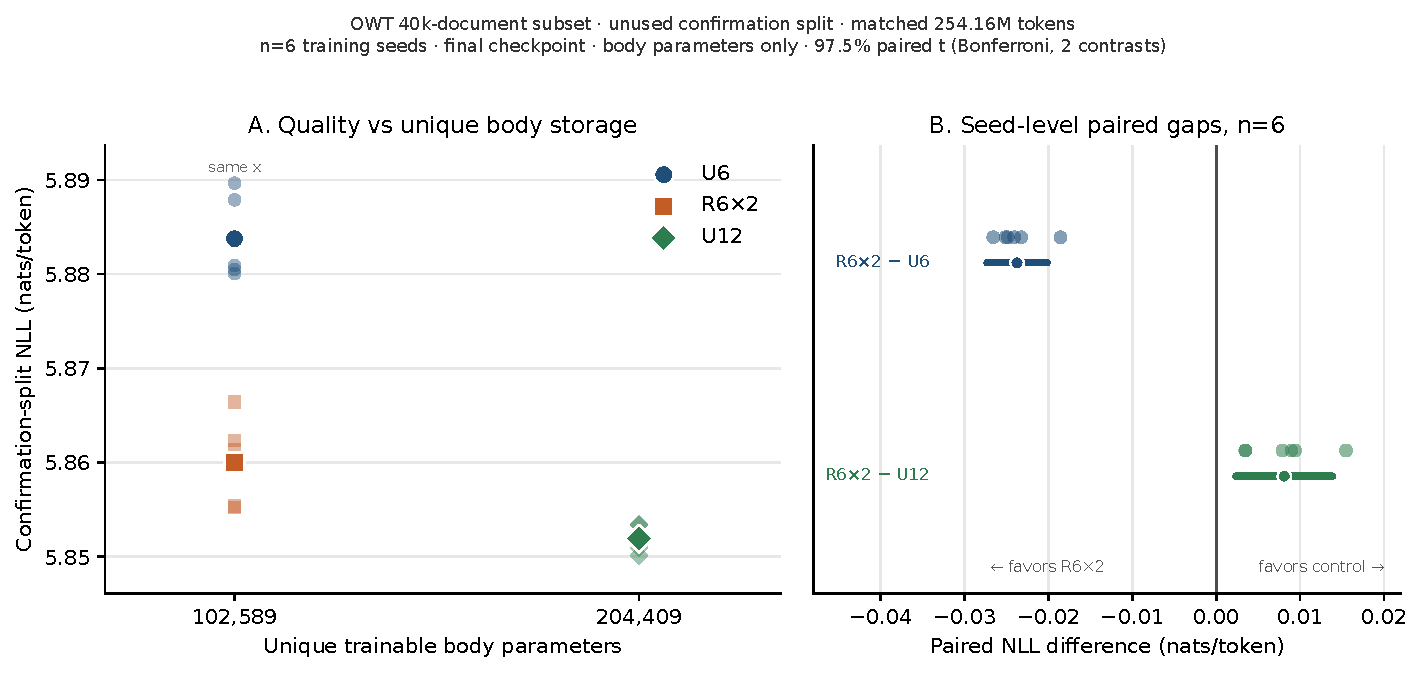
\includegraphics[width=\linewidth]{fig2-main-result.pdf}
\caption{Quality--storage trade-off on the confirmation holdout.
All models were trained for $254{,}164{,}992$ target-token presentations.
(a)~Final NLL versus unique trainable body parameters, excluding embedding and classifier;
faint markers denote six training seeds. U6 and R6$\times$2 share the $x$-coordinate.
(b)~Paired NLL differences between R6$\times$2 and each control, with individual seed
differences, means, and $97.5\%$ paired Student-$t$ intervals (Bonferroni over two contrasts).
Negative differences favor recurrence. Not a non-inferiority test; not pooled with
calibration or development runs.}
\label{fig:main-result}
\end{figure}

\begin{figure}[t]
\centering
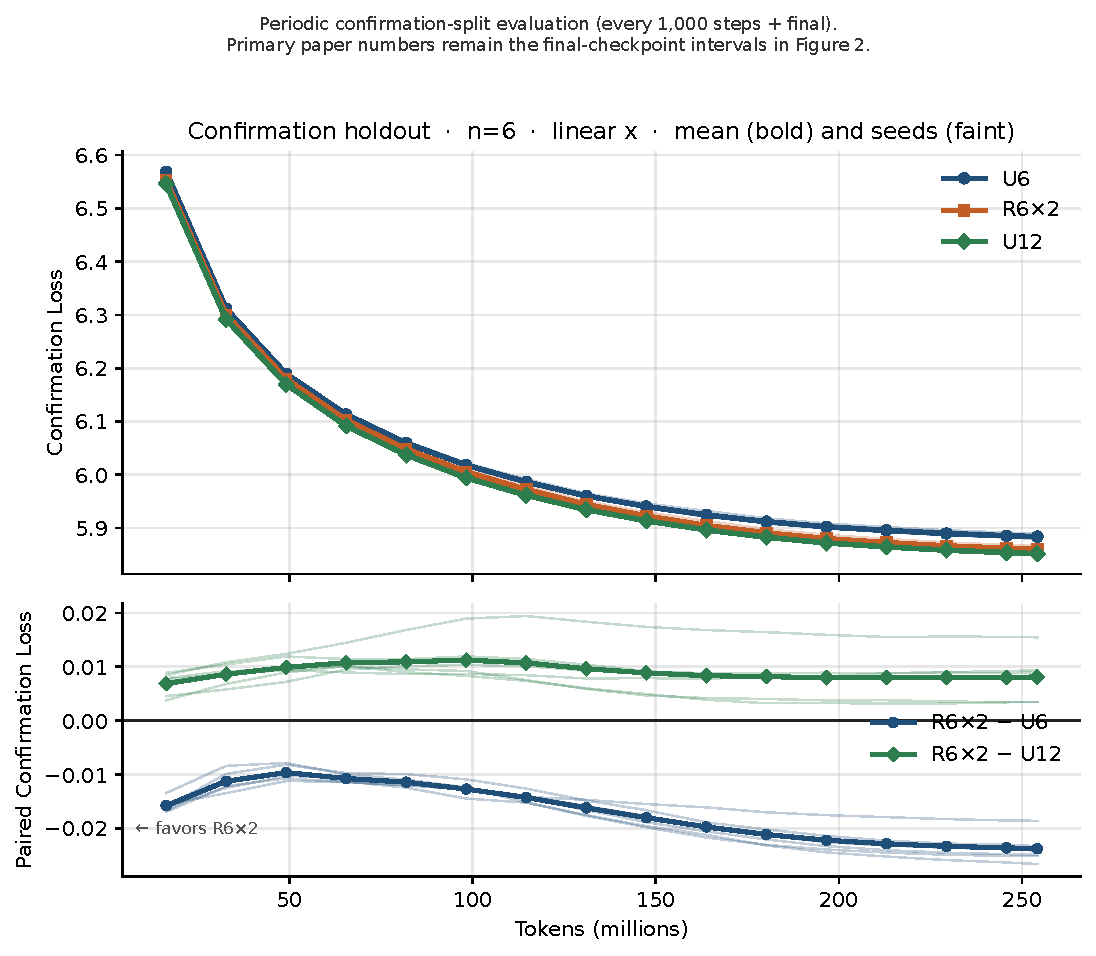
\includegraphics[width=\linewidth]{fig5-holdout-curves.pdf}
\caption{Confirmation-split NLL versus training-token presentations for six seeds.
Bold lines are means; faint lines are individual seeds. Lower panel: mean paired
gaps versus U6 and U12 (negative favors R6$\times$2). Evaluations every $1{,}000$ steps
plus the final checkpoint ($810{,}496$ scored tokens). Primary numerical claims remain
the final-checkpoint intervals; these trajectories are descriptive and were not used
for checkpoint selection.}
\label{fig:holdout-curves}
\end{figure}

\section{Conditional Hardware Analysis}

The experiments establish a quality--storage trade-off in software. This section asks when that trade-off \emph{could} matter on a capacity-limited thermodynamic sampling unit (TSU). It is not a measurement of TSU energy, latency, or mapping feasibility.

\paragraph{Mapping assumption.}
We assume each residual block can be mapped to a retained program on a compatible fabric that holds six complete block programs. Retaining neural weights does not necessarily eliminate input-conditioning or bias writes; independent sparse graphs may require routing or topology changes. Any such costs remain in the non-loading terms.

\paragraph{Schedule.}
Final norm, classifier, AFT histories, and workspace require separately accounted storage. Under a whole-bank, fixed-order replacement schedule for lockstep autoregressive decode:
\begin{itemize}
  \item U6 loads six blocks once and applies them once per token round;
  \item R6$\times$2 loads the same six blocks once and applies them twice per round;
  \item U12 loads blocks $1$--$6$, then replaces the bank with blocks $7$--$12$, every round.
\end{itemize}
Two U12 bank loads per round is a property of this schedule, not an optimal-cache lower bound. Batching, prefetching, partial retention, and teacher-forced prefill can change loading counts.

\paragraph{Three operating points.}
There is no single efficiency winner without a quality target and cost coefficients.

\begin{center}
\begin{tabular}{lccc}
\toprule
Model & Unique body & Applied depth & Loading under this schedule \\
\midrule
U6 & 6 blocks & 6 & resident after one load; less work than R6$\times$2 \\
R6$\times$2 & 6 blocks & 12 & resident after one load; more work than U6 \\
U12 & 12 blocks & 12 & two bank loads per decode round \\
\bottomrule
\end{tabular}
\end{center}

\paragraph{Energy accounting.}
For the R6$\times$2-versus-U12 comparison, let \(\varepsilon\) be energy per six-block bank load, \(Q_i\) all other energy per decode round (conditioning, readout, AFT-state movement, head, control, static), \(N\) the number of rounds, and \(b\) the decode batch. Then
\[
\bar E_{\mathrm{U12}} = \frac{2N\varepsilon + N Q_{\mathrm{U12}}}{Nb},
\qquad
\bar E_{\mathrm{R6}\times 2} = \frac{\varepsilon + N Q_{\mathrm{R}}}{Nb}.
\]
Recurrence uses less energy under this model iff
\[
Q_{\mathrm{R}}-Q_{\mathrm{U12}} < \bigl(2-\tfrac{1}{N}\bigr)\varepsilon:
\]
additional non-loading energy per round must be smaller than the avoided, amortized bank-loading energy. Quality remains unmatched. U6 is also resident and performs less work than R6$\times$2.

\begin{figure}[t]
\centering
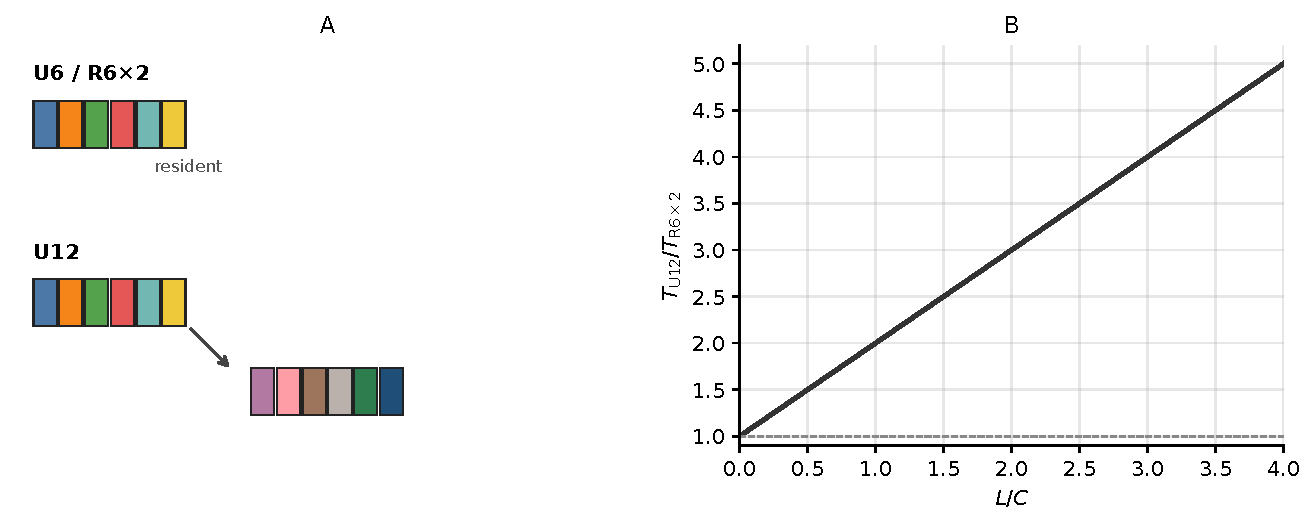
\includegraphics[width=\linewidth]{fig3-residency.pdf}
\caption{Conditional whole-bank replacement schedule if a fabric holds six block
programs. R6$\times$2 retains the bank; U12 loads two banks each decode round under
this schedule (not an optimal-cache bound). Panel B plots
\(\mathrm{speedup}=1+(\text{exposed U12 reload time})/(\text{common non-load compute})\)
assuming equal non-load compute. Not a TSU measurement. Observed quality is unmatched;
U6 is also weight-resident and performs less work.}
\label{fig:residency}
\end{figure}

\paragraph{What we do not claim.}
A high energy cost per coupling flash relative to one Gibbs update does not imply that programming dominates per-token energy for this model. Another neural-block application is not an extra Gibbs update under unchanged couplings and conditioning. We did not measure \(Q_{\mathrm{R}}-Q_{\mathrm{U12}}\). Observed quality is unmatched ($\approx 0.81\%$ extra perplexity versus U12). Extropic's published Z1 energy ordering (sample $\ll$ read $\ll$ flash)~\cite{amico2026} motivates treating unique-program size as first-class; it is not an evaluation of R6$\times$2. Quoted Z1T system energy remains dominated by host/FPGA orchestration in published figures, so moving only the sparse body on-chip need not make flashing the system bottleneck.

\section{Limitations and Conclusion}

Our findings are limited to one archived OpenWebText subset, one width and context length, and a shared training recipe rather than independently tuned models. The six-seed confidence intervals describe training variability conditional on a fixed evaluation corpus and do not capture uncertainty across datasets. Weight sharing reduces unique body parameters, not the embedding or classifier, and does not reduce applied depth relative to U12. We do not establish reasoning capability or improvements from increasing recurrence at inference without retraining.

The hardware analysis is a conditional cost model, not a measurement of TSU efficiency. We have not validated a resident hardware mapping, quantized sampling fidelity, or the programming, readout, state-transfer, and control costs of recurrent Z1T. In particular, another neural-block application is not equivalent to additional Gibbs updates under unchanged conditioning. Matched-quality sampling overhead is also unmeasured; the projected energy savings therefore remain hypotheses.

Within the tested regime, applying six shared blocks twice improves perplexity by $2.35\%$ over a six-block model, while approaching a twelve-block model with $49.8\%$ fewer unique body parameters and $0.81\%$ higher perplexity. This is a useful, but not lossless, quality--storage trade-off under the reported recipe and corpus. Additional applied computation can recover much of the benefit of additional unique depth. Whether that trade-off reduces TSU energy remains a question for measured mappings and coefficients.

\appendix
\section{Per-seed confirmation outcomes}

\begin{table}[h]
\centering
\caption{Per-seed final confirmation NLL (nats/token).}
\label{tab:per-seed-nll}
\begin{tabular}{crrrrr}
\toprule
Seed & U6 & R6$\times$2 & U12 & R6$\times$2 $-$ U12 & R6$\times$2 $-$ U6 \\
\midrule
7  & 5.883580 & 5.859483 & 5.850089 & $+0.009394$ & $-0.024097$ \\
8  & 5.887879 & 5.861300 & 5.853415 & $+0.007885$ & $-0.026580$ \\
9  & 5.880492 & 5.855362 & 5.851886 & $+0.003476$ & $-0.025130$ \\
10 & 5.880047 & 5.855187 & 5.851729 & $+0.003458$ & $-0.024860$ \\
11 & 5.889654 & 5.866393 & 5.850928 & $+0.015464$ & $-0.023261$ \\
12 & 5.880896 & 5.862328 & 5.853363 & $+0.008966$ & $-0.018567$ \\
\midrule
Mean & 5.883758 & 5.860009 & 5.851902 & $+0.008107$ & $-0.023749$ \\
\bottomrule
\end{tabular}
\end{table}

\section{Software environment}
\label{app:env}

All $18$ confirmation runs used NVIDIA H100 80GB HBM3 GPUs. Model arrays used float32 with \texttt{jax\_default\_matmul\_precision=None}. Recorded packages: Python $3.12.14$, JAX/jaxlib $0.11.1$, Equinox $0.13.8$, Optax $0.2.8$, NumPy $2.5.3$. Data identity: prepared-manifest SHA256 \texttt{53a5313d3fb3ae3a95e1a854d929524390e37ce05f32598e783e01014d3ce364}; source-document SHA256 \texttt{c98854af7dae63b01eaf03d29a1d6b66236b312b76ca928d6d7c75987474f588}. Tokenizer: GPT-2 BPE via tiktoken $0.12.0$; \texttt{encoder.json} SHA256 \texttt{196139668be63f3b5d6574427317ae82f612a97c5d1cdaf36ed2256dbf636783}; \texttt{vocab.bpe} SHA256 \texttt{1ce1664773c50f3e0cc8842619a93edc4624525b728b188a9e0be33b7726adc5}.

Checksummed metrics live in \texttt{artifacts/claim-a/}. Figures regenerate with \texttt{uv run python scripts/analyze\_claim\_a.py} and \texttt{uv run python scripts/make\_paper\_figures.py}. Full-state checkpoints are not in git. First-wave launcher provenance files inherit the label \texttt{duration-v1} from an earlier launcher; run configs and identities are claim-A. One registered U12 seed-$12$ run was retrained under the same identity after an infrastructure archive failure; it is not a replacement seed. Some earlier development checkpoints were not fully archived.

\section{Development history}
\label{app:history}

A toy character-level screen compared injection variants; residual input injection did not improve that set and was not used in the reported models. Short-horizon OpenWebText-subset runs established a small sharing cost at matched depth $12$ and motivated a six-block storage-matched control. An instrumented duration diagnostic (one development seed, matched tokens, periodic holdout evaluation) selected the $15{,}513$-step horizon. A three-seed calibration estimate on a previously unused calibration split assessed the same two contrasts. The original non-inferiority question at a $0.01$-nat margin was replaced by a trade-off estimate before the six-seed confirmation-split study; that study is the source of the main-text intervals.

\begin{thebibliography}{9}

\bibitem{dehghani2019}
Mostafa Dehghani, Stephan Gouws, Oriol Vinyals, Jakob Uszkoreit, and {\L}ukasz Kaiser.
\newblock Universal transformers.
\newblock In \emph{International Conference on Learning Representations}, 2019.

\bibitem{lan2020}
Zhenzhong Lan, Mingda Chen, Sebastian Goodman, Kevin Gimpel, Piyush Sharma, and Radu Soricut.
\newblock ALBERT: A lite BERT for self-supervised learning of language representations.
\newblock In \emph{International Conference on Learning Representations}, 2020.

\bibitem{geiping2025}
Jonas Geiping, Sean McLeish, Neel Jain, John Kirchenbauer, Siddharth Singh, Brian R.\ Bartoldson, Bhavya Kailkhura, Abhinav Bhatele, and Tom Goldstein.
\newblock Scaling up test-time compute with latent reasoning: A recurrent depth approach.
\newblock arXiv:2502.05171, 2025.

\bibitem{hao2024}
Shibo Hao, Sainbayar Sukhbaatar, DiJia Su, Xian Li, Zhiting Hu, Jason Weston, and Yuandong Tian.
\newblock Training large language models to reason in a continuous latent space.
\newblock arXiv:2412.06769, 2024.

\bibitem{zhai2021}
Shuangfei Zhai, Walter Talbott, Nitish Srivastava, Chen Huang, Hanlin Goh, Ruixiang Zhang, and Josh Susskind.
\newblock An attention free transformer.
\newblock arXiv:2105.14103, 2021.

\bibitem{zhu2025}
Jiachen Zhu, Xinlei Chen, Kaiming He, Yann LeCun, and Zhuang Liu.
\newblock Transformers without normalization.
\newblock In \emph{Proceedings of the IEEE/CVF Conference on Computer Vision and Pattern Recognition}, 2025.

\bibitem{extropic2026z1t}
Extropic.
\newblock Z1T.
\newblock \url{https://extropic.ai/writing/z1t/}, 2026.

\bibitem{amico2026}
Mirko Amico, Andra\v{z} Jelin\v{c}i\v{c}, Colin Oscar Nancarrow, Leo Tyrpak, David Roberts, Seth Morton, Dalton Sakthivadivel, Ashwin Gopal, and Guillaume Verdon.
\newblock Thermalizing stochastic programs.
\newblock arXiv:2608.01615v2, 2026.

\end{thebibliography}

\end{document}